\begin{frame}
	\frametitle{Traveling salesman problem}
	\begin{figure}
		\centering
		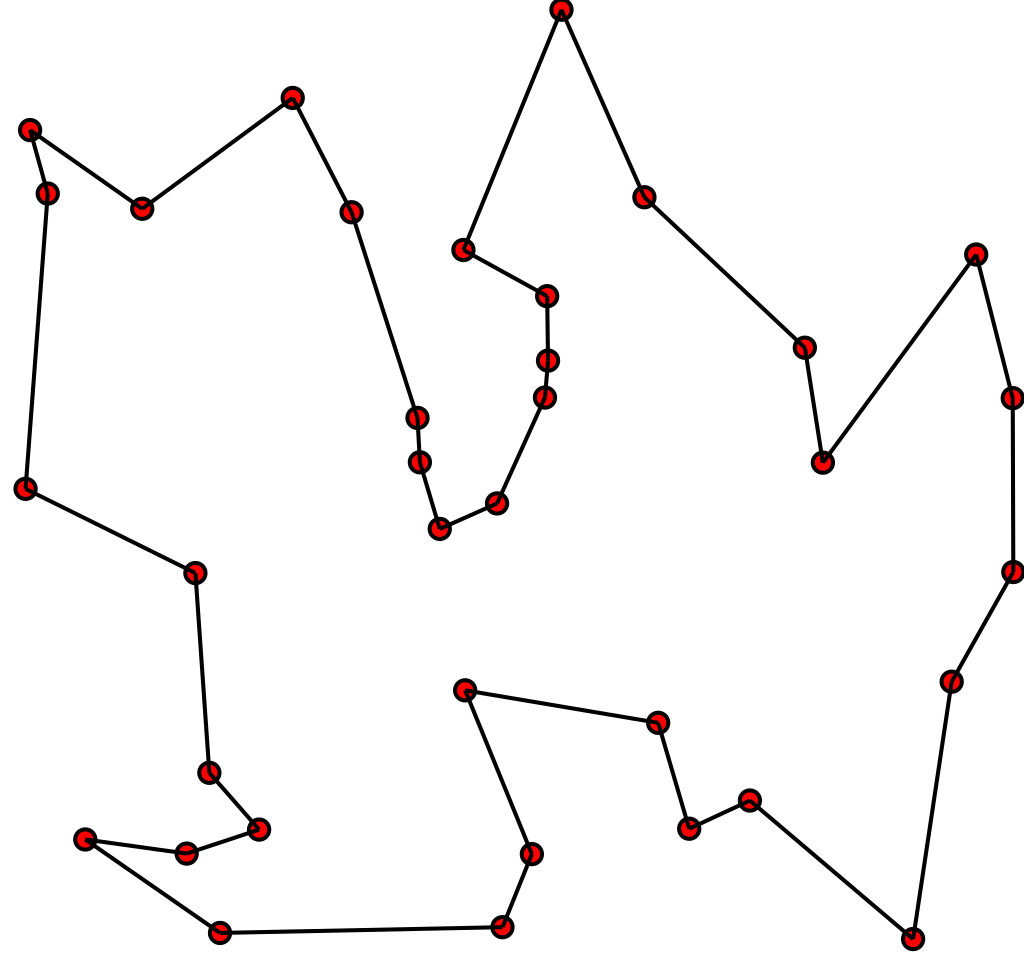
\includegraphics[scale=0.17]{img/travelling_salesman_problem}
		\caption{Traveling salesman problem, source: wiki.}
	\end{figure}
\end{frame}

\begin{frame}
	\frametitle{Traveling salesman problem}
	\begin{definition}
		A undirected graph $G$ is a pair $(V, E)$, where $V$ is a set of vertices and $E$ is a set of edges, which is a subset of all unordered pairs of vertices.
	\end{definition}
	\begin{definition}
		A tour is a Hamilitonian cycle and we identify it with a permutation of vertices.
	\end{definition}
\end{frame}

\begin{frame}
	\frametitle{Traveling salesman problem}
	\begin{definition}[Traveling salesman problem]
		Given an undirected weighted graph $G = (V, E)$, $|V| = n$ find a permutation $\sigma_{\min}$ of vertices such that
		\begin{equation*}
		\sigma_{\min} = \underset{\sigma \in S_n}{\argmin} \left( \sum_{i=1}^{n-1} w_{\sigma(i), \sigma(i+1)} + w_{\sigma(n), \sigma(1)} \right),
		\end{equation*}
		where $S_n$ is a set of all permutations of vertices and $w_{i,j}$ is distance (weight) between state i and j.
	\end{definition}
\end{frame}
